\documentclass[tikz,border=6pt]{standalone}
% Shared visual language for the original benchmark atlas.
\usepackage[T1]{fontenc}
\usepackage{lmodern}
\usepackage{amsmath,amssymb}
\usetikzlibrary{arrows.meta,calc,positioning,shapes.geometric,patterns,decorations.pathmorphing,backgrounds,fit}
\definecolor{ink}{HTML}{173948}
\definecolor{flow}{HTML}{167D9A}
\definecolor{control}{HTML}{A65217}
\definecolor{measure}{HTML}{70518A}
\definecolor{pale}{HTML}{EAF2F5}
\definecolor{muted}{HTML}{526571}
\definecolor{utility}{HTML}{2E8665}
\tikzset{
  every node/.style={font=\sffamily\small,text=ink},
  equipment/.style={draw=ink,line width=1pt,fill=pale,rounded corners=2pt},
  process/.style={draw=flow,line width=1.2pt,-{Latex[length=2.5mm]}},
  signal/.style={draw=control,line width=.8pt,dashed,-{Latex[length=2mm]}},
  util/.style={draw=utility,line width=1pt,-{Latex[length=2.2mm]}},
  dimension/.style={draw=muted,line width=.6pt,{Latex[length=1.7mm]}-{Latex[length=1.7mm]}},
  labelbox/.style={fill=white,inner sep=2pt,font=\sffamily\footnotesize,align=center},
  annotation/.style={font=\sffamily\footnotesize,text=muted,align=left},
  panel/.style={draw=ink!20,fill=ink!2,rounded corners=3pt,inner sep=6pt},
  instrument/.style={circle,draw=measure,fill=white,line width=.8pt,minimum size=8mm,inner sep=1pt,font=\sffamily\scriptsize,align=center},
  port/.style={circle,fill=flow,inner sep=1.6pt},
  box/.style={equipment,minimum width=3cm,minimum height=1cm,align=center},
}
\newcommand{\atlasheader}[3]{%
  \node[anchor=north west,font=\sffamily\bfseries\LARGE] at (0,0) {#1};%
  \node[anchor=north west,font=\sffamily\small,text=muted] at (0,-.75) {Paper section #2: \textit{#3}};%
  \draw[ink!25,line width=.7pt] (0,-1.25)--(26,-1.25);%
}
\newcommand{\atlasfooter}[1]{%
  \draw[ink!25,line width=.5pt] (0,-15.8)--(26,-15.8);%
  \node[anchor=north west,annotation,text width=25.8cm] at (0,-16) {#1\\Original explanatory drawing. Source: Kroll \& Schulte (2014), DOI: 10.1016/j.asoc.2014.08.034. Model variants are identified in the accompanying case sheet.};%
}

\usetikzlibrary{shadings,shadows,decorations.markings}
% Independent educational automotive throttle interpretation, section 3.4.
% Atmospheric engine-test-cell elements are decorative, not benchmark hardware.
% All models, units and signal directions retain the established atlas convention.
\definecolor{charcoal}{HTML}{34424A}
\definecolor{graphite}{HTML}{26343C}
\definecolor{steelEdge}{HTML}{53676F}
\definecolor{steelShade}{HTML}{849BA4}
\definecolor{steelMid}{HTML}{C4D3D5}
\definecolor{steelHi}{HTML}{FCFAF1}
\definecolor{pearl}{HTML}{EEF2ED}
\definecolor{blueMotor}{HTML}{396D85}
\definecolor{blueMotorLight}{HTML}{73A1A9}
\definecolor{blueMotorDark}{HTML}{254D64}
\definecolor{airDeep}{HTML}{137DAB}
\definecolor{airLight}{HTML}{5DC5DD}
\definecolor{amber}{HTML}{CC782E}
\definecolor{amberLight}{HTML}{F5C06B}
\definecolor{bronze}{HTML}{C39A67}
\definecolor{bronzeShadow}{HTML}{79543D}
\definecolor{copper}{HTML}{D68D55}
\definecolor{boardGreen}{HTML}{5C937B}
\definecolor{boardDeep}{HTML}{366A62}
\definecolor{violet}{HTML}{7D619B}
\definecolor{bench}{HTML}{5B6060}
\definecolor{benchHi}{HTML}{A4A8A0}
\definecolor{warmWall}{HTML}{EEE8D9}
\definecolor{coolWall}{HTML}{D8E4E6}
\definecolor{workLight}{HTML}{FFF3DC}
\definecolor{darkBore}{HTML}{718791}
\definecolor{boreLight}{HTML}{E5F1F0}
\definecolor{panelWarm}{HTML}{F9F4E9}
\definecolor{panelBlue}{HTML}{ECF3F4}
\tikzset{
  every node/.style={font=\sffamily\small,text=ink},
  airarrow/.style={draw=airDeep,line width=1.45pt,line cap=round,-{Triangle[length=2.8mm,width=2.1mm]}},
  powerline/.style={draw=boardDeep,line width=1.35pt,line cap=round,-{Triangle[length=2.6mm,width=1.8mm]}},
  cmdline/.style={draw=amber,line width=.97pt,dash pattern=on 3.5pt off 2.3pt,line cap=round,-{Triangle[length=2.2mm,width=1.5mm]}},
  sensline/.style={draw=violet,line width=.97pt,dash pattern=on 3.5pt off 2.3pt,line cap=round,-{Triangle[length=2.2mm,width=1.5mm]}},
  labelglass/.style={font=\sffamily\footnotesize,fill=white,fill opacity=.94,text opacity=1,rounded corners=1.0pt,inner xsep=3pt,inner ysep=2pt,align=center},
  technical/.style={panel,draw=steelEdge!23,fill=panelBlue},
}
\begin{document}
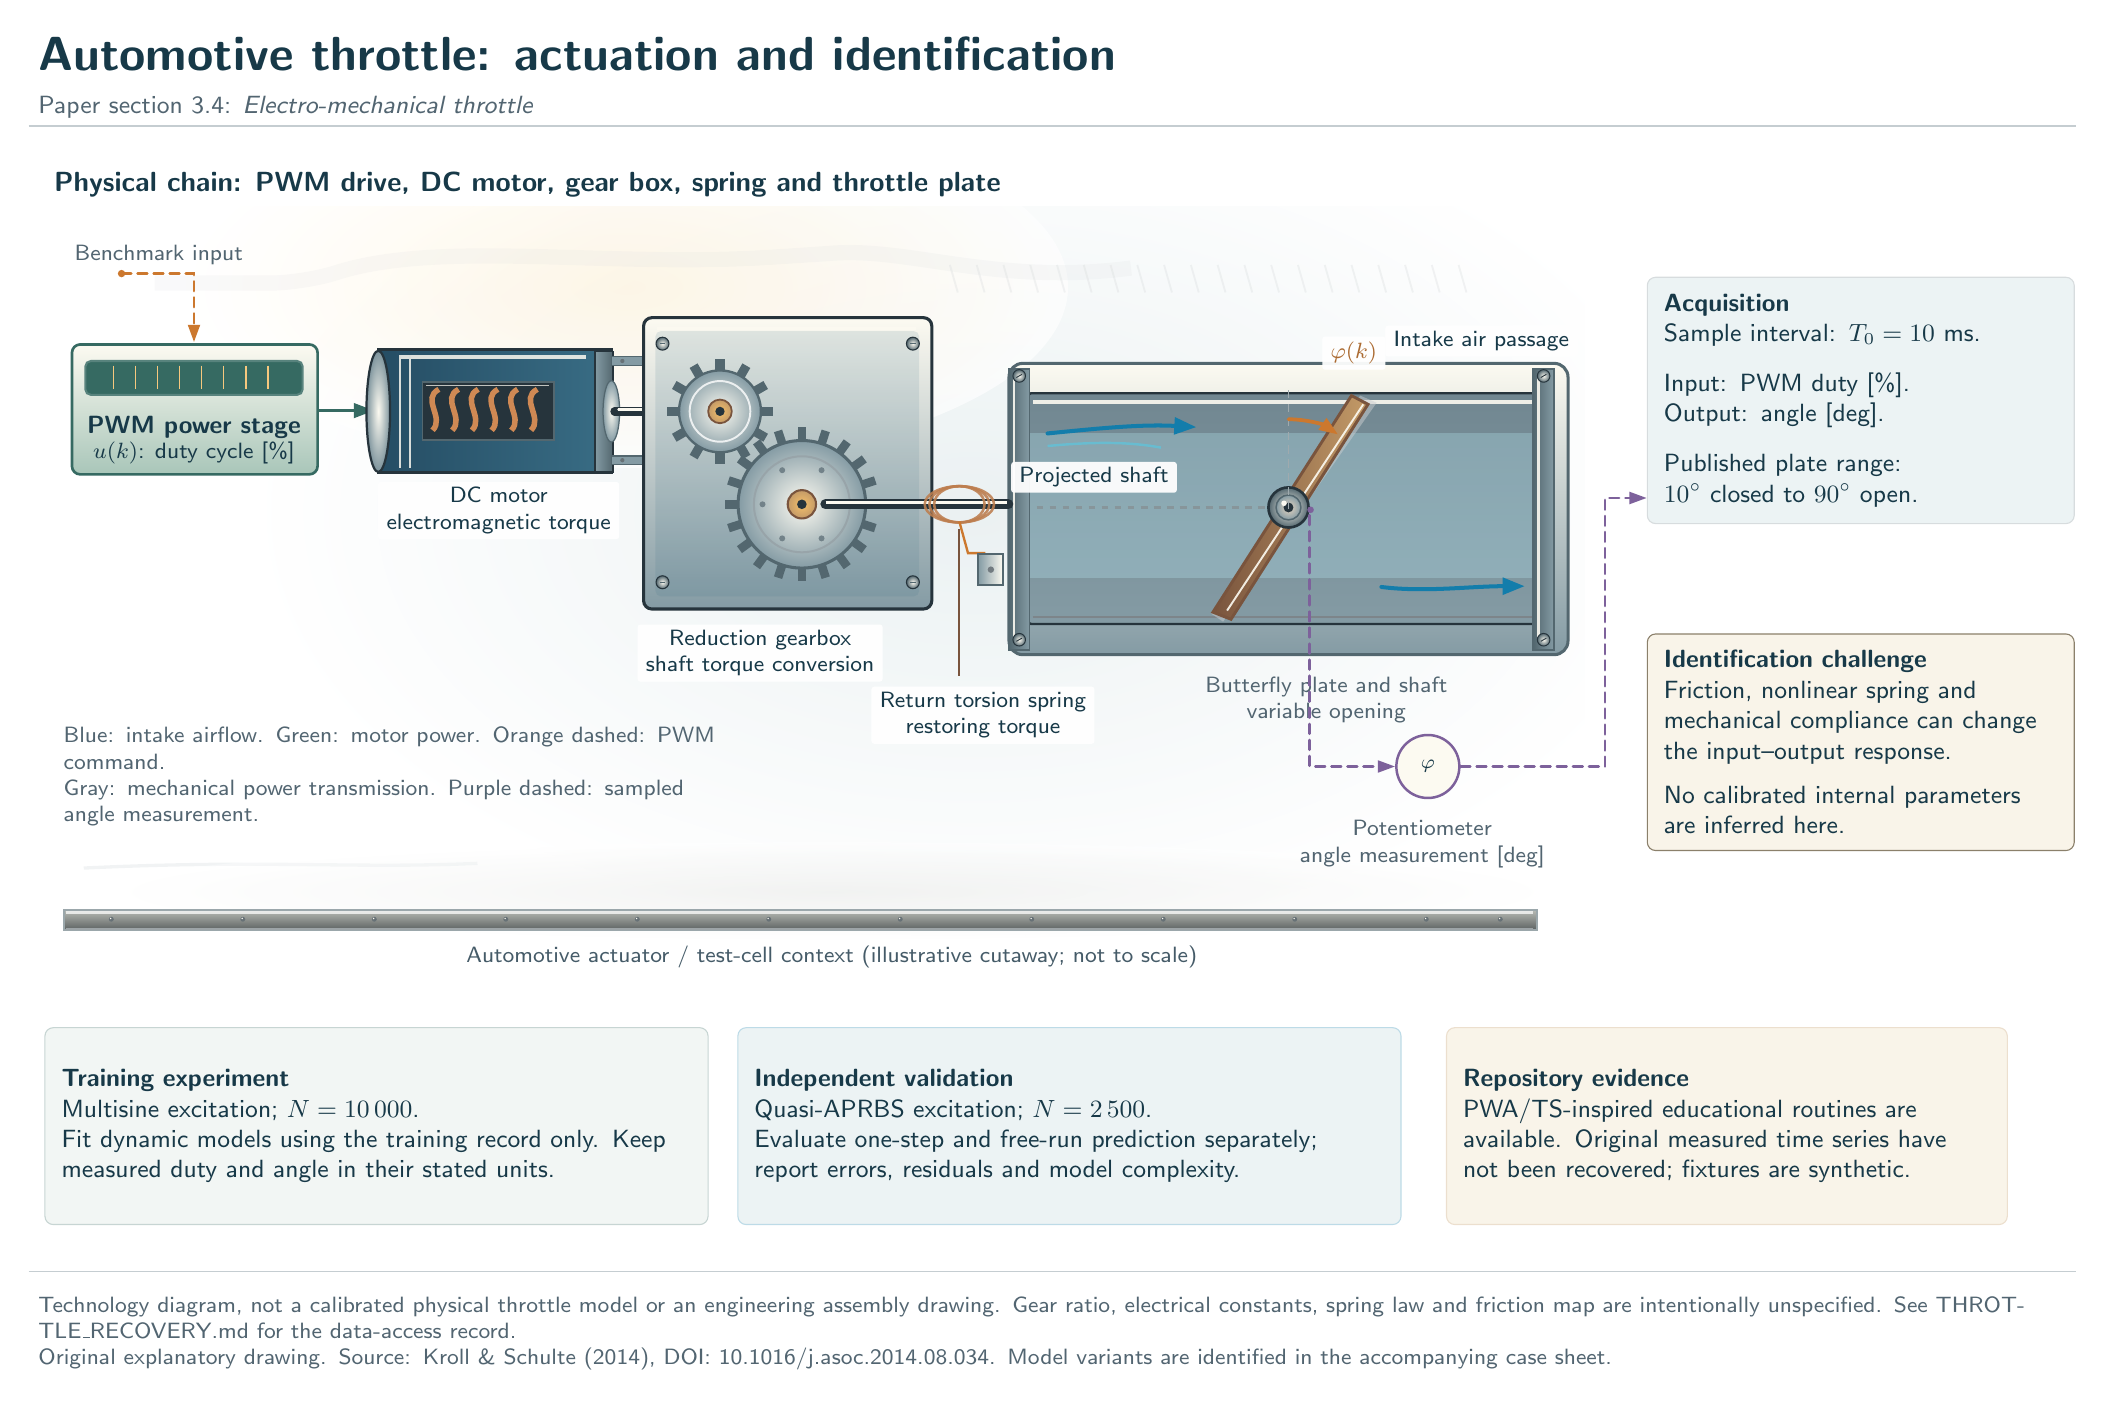
\begin{tikzpicture}[x=1cm,y=1cm]
\atlasheader{Automotive throttle: actuation and identification}{3.4}{Electro-mechanical throttle}
\node[anchor=west,font=\sffamily\bfseries] at (.2,-2.0)
 {Physical chain: PWM drive, DC motor, gear box, spring and throttle plate};

% ENGINE-TEST-CELL AMBIENCE. Soft defocused body panels, overhead light and
% shaded instrument plinth give physical context without imitating a landscape.
% Intentional no extraneous measured variables, badges or instrument icons.
\begin{scope}
 \clip (.13,-2.28) rectangle (19.76,-11.94);
 \shade[inner color=coolWall,outer color=white,opacity=.52]
   (12.0,-6.15) ellipse (9.1cm and 5.4cm);
 \shade[inner color=workLight,outer color=white,opacity=.66]
   (7.6,-3.30) ellipse (5.6cm and 2.3cm);
 % Engine test-cell housing, distant curved duct line (not a process connection).
 \draw[graphite!17,line width=5.5pt,opacity=.16,rounded corners=12pt]
  (1.6,-3.25)--(3.5,-3.25)..controls(5.2,-2.7)and(7.3,-3.05)..(9.8,-2.9)
  ..controls(11.2,-2.8)and(12.3,-3.28)..(14.0,-3.06);
 \draw[steelShade!65,line width=1.2pt,opacity=.18]
  (.7,-10.68)..controls(3,-10.57)and(4.1,-10.69)..(5.7,-10.62);
 % Faint industrial vent ribs, pushed behind the actuator.
 \foreach \xx in {11.70,12.04,12.38,12.72,13.06,13.40,13.74,14.08,14.42,14.76,15.10,15.44,15.78,16.12,16.46,16.80,17.14,17.48,17.82,18.16}{
   \draw[charcoal!18,line width=.68pt,opacity=.35] (\xx,-3.02)--(\xx+.1,-3.37);
 }
 \shade[inner color=benchHi!38!white,outer color=white,opacity=.36]
   (10.2,-10.98) ellipse (9.3cm and .63cm);
\end{scope}
% Underlying machined aluminum test platen, left deliberately low-contrast.
\shade[draw=steelEdge!58,line width=.7pt,
  top color=benchHi!78!white,middle color=benchHi,bottom color=bench]
  (.45,-11.21) rectangle (19.15,-11.47);
\draw[white,line width=.85pt,opacity=.72] (.48,-11.245)--(19.11,-11.245);
\draw[graphite!45,line width=.65pt] (.47,-11.45)--(19.10,-11.45);
\foreach \xx in {1.05,2.72,4.39,6.06,7.73,9.40,11.07,12.74,14.41,16.08,17.75,18.69}{
  \fill[graphite!70] (\xx,-11.33) circle (.031);
  \fill[steelHi!92!white] (\xx-.008,-11.32) circle (.010);
}
\node[anchor=north,annotation,text=muted!78!ink] at (10.2,-11.55)
 {Automotive actuator / test-cell context (illustrative cutaway; not to scale)};

% POWER STAGE: a distinct electronic module with translucent green cover,
% connector, miniature board and identified benchmark input u(k).
\shade[draw=boardDeep,line width=.96pt,rounded corners=3pt,
 top color=steelHi,middle color=panelBlue,bottom color=boardGreen!53!white]
  (.55,-4.03) rectangle (3.67,-5.68);
\shade[draw=boardDeep!83,line width=.75pt,rounded corners=2pt,
 left color=boardDeep,middle color=boardGreen,right color=boardDeep]
  (.72,-4.24) rectangle (3.48,-4.67);
\foreach \xx in {1.08,1.36,1.64,1.92,2.20,2.48,2.76,3.04}{
 \draw[amberLight!87!white,line width=.40pt] (\xx,-4.30)--(\xx,-4.59);
}
\node[font=\sffamily\small,align=center] at (2.10,-5.08) {\textbf{PWM power stage}};
\node[font=\sffamily\footnotesize,align=center] at (2.10,-5.41) {$u(k)$: duty cycle [\%]};
% Stable incoming command: begins at a clearly marked source marker.
\node[anchor=west,annotation] at (.46,-2.89) {Benchmark input};
\fill[amber] (1.18,-3.13) circle (.047);
\draw[cmdline] (1.18,-3.13)--(2.10,-3.13)--(2.10,-4.00);
\draw[powerline] (3.69,-4.87)--(4.39,-4.87);

% MOTOR: graphite-blue cylindrical can with copper windings and brushed cap.
% Three-dimensional shading is explanatory, not a manufacturer cutaway.
\shade[draw=graphite,line width=1.06pt,
  left color=blueMotorDark,middle color=blueMotorLight,right color=blueMotor]
 (4.44,-4.10) rectangle (7.40,-5.66);
\shade[draw=graphite,line width=.8pt,
 inner color=steelHi,outer color=steelShade!85!steelEdge]
 (4.44,-4.88) ellipse (.15cm and .77cm);
\shade[draw=graphite,line width=.66pt,left color=steelShade,
 middle color=steelHi,right color=steelEdge]
 (7.19,-4.12) rectangle (7.42,-5.65);
\draw[steelHi,line width=1.20pt,opacity=.85] (4.73,-4.19)--(7.08,-4.19);
% Motor rotor/copper coils glimpsed through a service opening.
\shade[draw=steelEdge,line width=.6pt,left color=graphite,
 middle color=steelShade,right color=graphite]
 (5.00,-4.51) rectangle (6.67,-5.24);
\foreach \xx in {5.13,5.38,5.63,5.88,6.13,6.38}{
 \draw[copper,line width=2.0pt,opacity=.96]
  (\xx,-5.12)..controls(\xx+.16,-4.96)and(\xx-.15,-4.72)..(\xx+.08,-4.60);
}
\draw[steelHi,line width=.43pt,opacity=.72] (5.05,-4.55)--(6.61,-4.55);
\foreach \xx in {4.72,4.84}{
 \draw[steelHi!70!steelShade,line width=.64pt] (\xx,-4.17)--(\xx,-5.60);
}
\shade[draw=steelEdge,line width=.45pt,inner color=steelHi,outer color=steelShade]
 (7.40,-4.88) ellipse (.105cm and .39cm);
\draw[graphite,line width=3.0pt,line cap=round] (7.44,-4.88)--(8.81,-4.88);
\draw[steelHi,line width=.84pt,line cap=round] (7.49,-4.855)--(8.81,-4.855);
\node[anchor=north,labelglass] at (5.97,-5.77) {DC motor \\ electromagnetic torque};

% Motor-can retaining brackets meet the gearbox shell; they are not a signal.
\foreach \yy in {-4.24,-5.50}{
 \shade[draw=steelEdge,line width=.53pt,left color=steelShade,
  middle color=steelHi,right color=steelShade]
  (7.40,\yy-.055) rectangle (7.85,\yy+.055);
 \fill[graphite!70] (7.54,\yy) circle (.027);
}
% REDUCTION TRANSMISSION: enclosed gearbox with visible steel gears and
% copper-colored center bosses. Their teeth are simple geometric approximations.
\shade[draw=graphite,line width=1.12pt,rounded corners=3pt,
 top color=steelHi,middle color=steelMid,bottom color=steelShade]
 (7.81,-3.69) rectangle (11.47,-7.39);
\path[fill=blueMotor,opacity=.13,rounded corners=2pt]
 (7.96,-3.86) rectangle (11.31,-7.23);
\draw[steelHi,line width=.9pt,opacity=.85] (7.98,-3.83)--(11.27,-3.83);
% Cover fasteners and machined corners.
\foreach \xx/\yy in {8.05/-4.02,11.23/-4.02,8.05/-7.05,11.23/-7.05}{
 \shade[draw=graphite,line width=.39pt,inner color=steelHi,outer color=steelEdge]
   (\xx,\yy) circle (.082);
 \draw[steelEdge,line width=.38pt] (\xx-.035,\yy)--(\xx+.035,\yy);
}
\foreach \a in {0,30,...,330}{
  \draw[steelEdge,line width=3.3pt] ($(8.78,-4.88)+(\a:.50)$)--($(8.78,-4.88)+(\a:.67)$);
}
\shade[draw=steelEdge,line width=.85pt,inner color=steelHi,outer color=steelShade]
 (8.78,-4.88) circle (.52);
\draw[white,line width=.7pt,opacity=.80] (8.78,-4.88) circle (.385);
\shade[draw=bronzeShadow,line width=.65pt,inner color=amberLight,outer color=bronze]
 (8.78,-4.88) circle (.15);
\fill[graphite] (8.78,-4.88) circle (.059);
\foreach \a in {0,18,...,342}{
  \draw[steelEdge,line width=3.1pt] ($(9.82,-6.06)+(\a:.78)$)--($(9.82,-6.06)+(\a:.98)$);
}
\shade[draw=steelEdge,line width=1.10pt,inner color=steelHi,outer color=steelShade]
 (9.82,-6.06) circle (.81);
\draw[steelEdge!60,line width=.72pt] (9.82,-6.06) circle (.61);
\foreach \a in {0,60,...,300}{
 \fill[steelEdge!82] ($(9.82,-6.06)+(\a:.50)$) circle (.038);
}
\shade[draw=bronzeShadow,line width=.75pt,inner color=amberLight,outer color=bronze]
 (9.82,-6.06) circle (.18);
\fill[graphite] (9.82,-6.06) circle (.061);
\node[anchor=north,labelglass,align=center] at (9.29,-7.58) {Reduction gearbox \\ shaft torque conversion};

% FLOW BODY: dark outer casting, dimensioned aluminum flange rings,
% atmospheric intake bore, and a single physically hinged butterfly plate.
% The split long-section is schematic; no unmeasured flow rate is asserted.
\shade[draw=steelEdge,line width=1.10pt,rounded corners=5pt,
 top color=steelHi,middle color=steelMid,bottom color=steelShade]
 (12.45,-4.27) rectangle (19.55,-7.97);
\shade[draw=graphite,line width=.88pt,rounded corners=2pt,
 top color=darkBore,middle color=boreLight,bottom color=steelShade]
 (12.66,-4.65) rectangle (19.36,-7.58);
\path[fill=airLight!45!white,opacity=.30]
 (12.67,-5.16)--(19.36,-5.16)--(19.36,-6.99)--(12.67,-6.99)--cycle;
\draw[steelHi,line width=1.20pt,opacity=.90] (12.76,-4.76)--(19.24,-4.76);
\draw[graphite!60,line width=.80pt] (12.75,-7.49)--(19.28,-7.49);
% Flange collars raised from the casting, with distinct bolt heads.
\foreach \xx in {12.58,19.24}{
 \shade[draw=steelEdge,line width=.64pt,left color=steelEdge,
 middle color=steelHi,right color=steelShade]
  (\xx-.13,-4.34) rectangle (\xx+.13,-7.91);
 \draw[steelHi,line width=.76pt,opacity=.9] (\xx-.065,-4.46)--(\xx-.065,-7.74);
 \foreach \yy in {-4.43,-7.78}{
  \shade[draw=graphite,line width=.35pt,inner color=steelHi,outer color=steelEdge]
   (\xx,\yy) circle (.080);
  \draw[graphite,line width=.32pt] (\xx-.036,\yy-.020)--(\xx+.035,\yy+.020);
 }
}
\node[anchor=south,labelglass] at (18.45,-4.19) {Intake air passage};
% Blue streamlines follow the open portion, distinct from motor command.
\draw[airarrow] (12.94,-5.16)..controls(13.55,-5.10)and(14.12,-5.04)..(14.83,-5.08);
\draw[airarrow] (17.18,-7.11)..controls(17.73,-7.18)and(18.31,-7.10)..(19.00,-7.10);
\draw[airLight,line width=.88pt,opacity=.72]
 (12.94,-5.32)..controls(13.57,-5.26)and(14.00,-5.27)..(14.38,-5.34);
% Continuity between gear output and throttle shaft; inside the bore the
% axial projection is dashed to avoid claiming a visible free-running bar.
\draw[graphite,line width=3.7pt,line cap=round] (10.12,-6.06)--(12.44,-6.06);
\draw[steelHi,line width=1.00pt] (10.12,-6.035)--(12.43,-6.035);
\draw[steelEdge!70,dash pattern=on 2.5pt off 2.2pt,line width=.79pt]
 (12.80,-6.10)--(15.73,-6.10);
\node[anchor=south,labelglass] at (13.53,-5.92) {Projected shaft};
% Butterfly plate is rendered as a slim, continuous swept metal surface.
\path[fill=graphite!24,opacity=.50]
 (15.02,-7.45)--(15.17,-7.55)--(17.12,-4.77)--(16.91,-4.68)--cycle;
\shade[draw=bronzeShadow,line width=1.05pt,
 left color=bronzeShadow,middle color=amberLight,right color=bronze]
 (15.04,-7.43)--(15.27,-7.52)--(17.01,-4.79)--(16.80,-4.68)--cycle;
\draw[steelHi,line width=.69pt,opacity=.91] (15.22,-7.41)--(16.95,-4.79);
\shade[draw=graphite,line width=.94pt,inner color=steelHi,outer color=steelEdge]
 (16,-6.10) circle (.255);
\shade[draw=steelEdge,line width=.55pt,inner color=bronze!40!white,outer color=steelShade]
 (16,-6.10) circle (.158);
\fill[graphite] (16,-6.10) circle (.063);
\fill[steelHi] (15.943,-6.047) circle (.035);
\node[anchor=north,annotation,align=center,text width=3.9cm] at (16.48,-8.13)
 {Butterfly plate and shaft \\ variable opening};
% Actual reference axis through pivot, and one exact-angle arc (no drift).
\draw[steelEdge!56,dash pattern=on 3pt off 2pt,line width=.72pt]
 (16,-6.12)--(16,-4.56);
\draw[amber,line width=1.35pt,line cap=round,
 -{Triangle[length=2.4mm,width=1.7mm]}]
 (16,-4.98) arc[start angle=90,end angle=55.8,radius=1.12];
\node[labelglass,text=amber!80!graphite] at (16.83,-4.14) {$\varphi(k)$};

% TORSIONAL RETURN SPRING: concentric around the output shaft; unlike an
% arbitrary extension spring this depicts restoring torque at the same axis.
\foreach \rr in {.32,.38,.44}{
 \draw[copper!73!bronzeShadow,line width=.92pt,opacity=.88]
  (11.82,-6.06) ellipse (\rr cm and .23cm);
}
\draw[amber,line width=.85pt] (11.82,-6.28)--(11.93,-6.68)--(12.15,-6.68);
\shade[draw=steelEdge,line width=.68pt,left color=steelShade,right color=steelHi]
 (12.06,-6.69) rectangle (12.37,-7.09);
\fill[graphite!65] (12.22,-6.89) circle (.041);
\draw[bronzeShadow,line width=.71pt] (11.82,-6.37)--(11.82,-8.24);
\node[anchor=north,labelglass,align=center] at (12.12,-8.37)
 {Return torsion spring \\ restoring torque};

% POTENTIOMETER OUTPUT: explicit physical junction, separate from blue airflow.
\fill[violet] (16.28,-6.13) circle (.042);
\node[instrument,draw=violet,fill=steelHi,line width=.90pt] (sensor) at (17.77,-9.39) {$\varphi$};
\draw[sensline] (16.27,-6.20)--(16.27,-9.39)--(sensor.west);
\node[anchor=north,annotation,text width=4.2cm,align=center] at (17.70,-9.95)
 {Potentiometer \\ angle measurement [deg]};
\draw[sensline] (sensor.east)--(20.02,-9.39)--(20.02,-5.98)--(20.55,-5.98);

% Explanatory signal legend, positioned without touching hardware.
\node[annotation,anchor=west,text width=8.45cm] at (.32,-9.52)
 {Blue: intake airflow. Green: motor power. Orange dashed: PWM command. \\ Gray: mechanical power transmission. Purple dashed: sampled angle measurement.};

% Model statements and evaluation commitments carried over from the atlas.
\hyphenpenalty=10000\exhyphenpenalty=10000\emergencystretch=1em
\node[technical,anchor=north west,text width=5cm,align=left] (acq) at (20.55,-3.17)
 {\textbf{Acquisition}\\Sample interval: $T_0=10$ ms.\\[7pt]
 Input: PWM duty [\%].\\Output: angle [deg].\\[7pt]
 Published plate range:\\$10^\circ$ closed to $90^\circ$ open.};
\node[panel,draw=bronze!50!steelEdge,fill=panelWarm,
 anchor=north west,text width=5cm,align=left] at (20.55,-7.7)
 {\textbf{Identification challenge}\\Friction, nonlinear spring and
 mechanical compliance can change the input--output response.\\[5pt]
 No calibrated internal parameters are inferred here.};
\node[panel,draw=boardDeep!28,fill=boardGreen!8!white,
 anchor=north west,text width=8cm,minimum height=2.5cm,align=left] at (.2,-12.7)
 {\textbf{Training experiment}\\Multisine excitation; $N=10\,000$.\\
 Fit dynamic models using the training record only. Keep measured duty
 and angle in their stated units.};
\node[panel,draw=airDeep!28,fill=panelBlue,
 anchor=north west,text width=8cm,minimum height=2.5cm,align=left] at (9,-12.7)
 {\textbf{Independent validation}\\Quasi-APRBS excitation; $N=2\,500$.\\
 Evaluate one-step and free-run prediction separately; report errors,
 residuals and model complexity.};
\node[panel,draw=bronze!32,fill=panelWarm,
 anchor=north west,text width=6.7cm,minimum height=2.5cm,align=left] at (18,-12.7)
 {\textbf{Repository evidence}\\PWA/TS-inspired educational routines are
 available. Original measured time series have not been recovered;
 fixtures are synthetic.};
\hyphenpenalty=50\exhyphenpenalty=50\emergencystretch=0pt
\atlasfooter{Technology diagram, not a calibrated physical throttle model or an engineering assembly drawing. Gear ratio, electrical constants, spring law and friction map are intentionally unspecified. See THROTTLE\_RECOVERY.md for the data-access record.}
\end{tikzpicture}
\end{document}
